\chapter{Arbetet}
\label{sec:arbetet}
Arbetet kan del


Stort problem är att json och json scheman inte skiljer på heltal och reela tal, medan många språk gör det. Specifikt Delphi som systemet utvecklades i.

\section{Systemet i helhet}

När användargränssnittet ska visas första gången, eller efter att en användare valt att trycka på "spara-knappen" (se figur \ref{label}), skickar servern två dokument till klienten. Det dataflödet illustreras i figur \ref{fig:system:ner}. Det ena dokumentet är ett JSON Schema som beskriver vilken data användaren med hjälp av klienten ska kunna se och redigera. Det andra dokumentet som skickas till klienten är den faktiska data som är sparad på servern. Först så parsas schemat och representeras i instanser av \textit{records} eller objekt i Delphi. Sedan används datan för att populera objekten med de korrekta värdena, för att tillsammans skapa modellen. Det sista steget är att det grafiska användargränssnittet genereras och presenteras för användaren.

Varje gång användaren interagerar med användargränssnittet och matar in giltig data, uppdateras modellen vilket i sin tur uppdaterar det grafiska användargränssnittet. Det dataflödet illustreras i figur \ref{fig:system:upp} Detta sker utan någon kontakt med servern. Om användaren är nöjd med sina ändringar och vill spara dem på servern kan användaren trycka på "spara-knappen" (se figur \ref{label}) så uppdateras dataobjektet med de nya värdena från datamodellen, vilket sedan skickas till servern. Efter det börjar systemet igång från början igen.

\begin{figure}
	\begin{subfigure}{0.5\textwidth}
		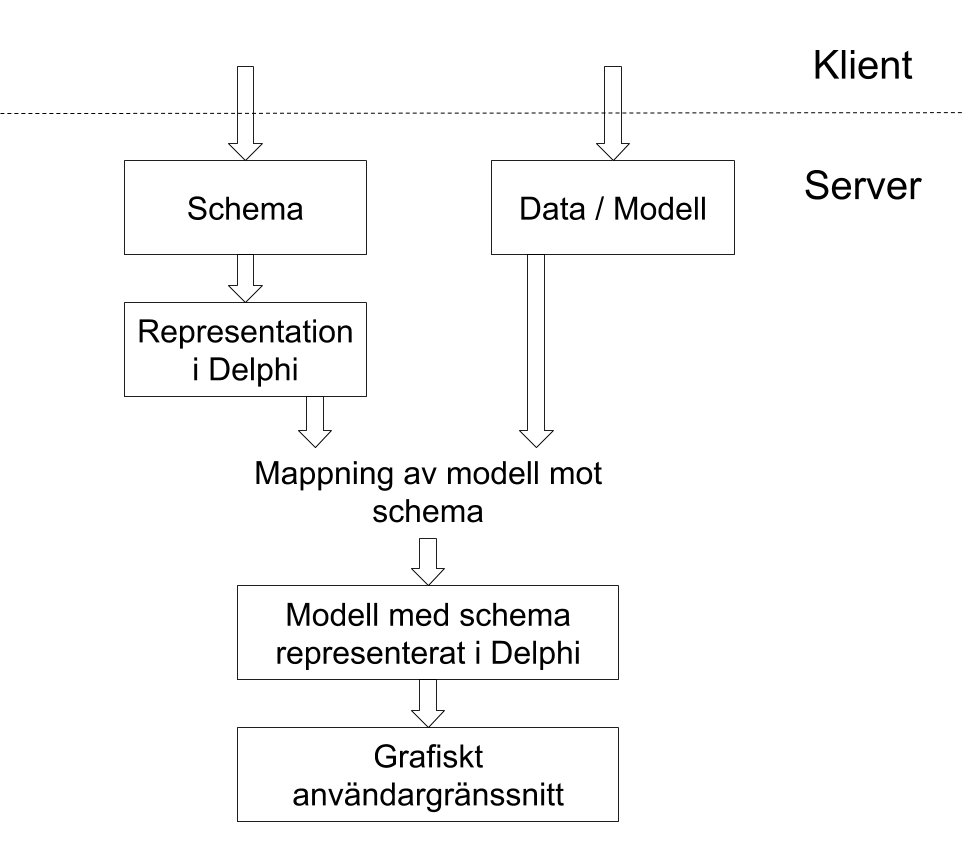
\includegraphics[width=0.9\textwidth,left]{./images/system-ner.png}
		\caption{Flödesschema över systemet}
		\label{fig:system:ner}
	\end{subfigure}
	\begin{subfigure}{0.5\textwidth}
		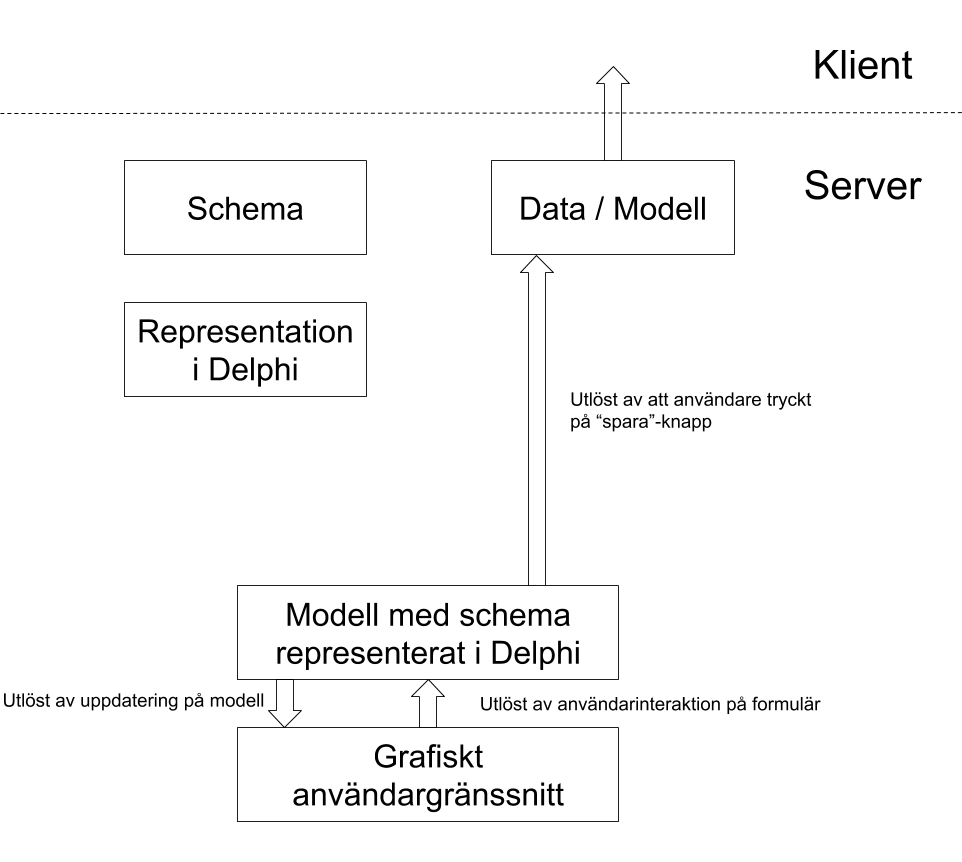
\includegraphics[width=0.9\textwidth,right]{./images/system-upp.png}
		\caption{Flödesschema över systemet}
		\label{fig:system:upp}	
	\end{subfigure}
	\caption{Illustration av dataflöde till och från användargränssnittet}
	\label{fig:system}
\end{figure}

\section{Generering av JSON Schema i Delphi}

Hur JSON Schemat genereras, påverkar inte slutanvändaren, men det påverkar utvecklarna som ska jobba med systemet, och kan hindra vilken funktionalitet som finns tillgänglig i systemet. Ett alternativ är självklart att skriva scheman för hand, men då olika klienter måste ha olika scheman, måste utvecklare se till att rätt schema hamnar på rätt klient vid instalationen av Mimer SoftRadio. Om en kund skulle vilja uppgradera funktionaliteten hos sin installation av Mimer SoftRadio, och därmed behöva tillgång till fler konfigurerbara inställningar i systemet, skulle schemat behöva uppdateras efteråt.

Ett annat alternativ är att basera schemat på inbyggda datatyper i det statiskt typade språket Delphi. Json.NET Schema, NJsonSchema for .NET, typescript-json-schema samt Typson erbjuder exakt den här funktionaliteten i språken .NET respektive TypeScript. För att lägga till extra beskrivningar av datan som språket inte räcker till för, använder .NET-implementationerna \textit{Data Annotation Attributes}, och TypeScript-implementationerna använder experimentella \textit{Decorators}. \cite{Suter,Newtonsoft,El-Dardiry,Bovet} Delphi erbjuder liknande funktionalitet med \textit{Attributes (RTTI)} \cite{Embarcadero2016}. Att annotera datastrukturerna som faktiskt sedan kommer användas i ett system kan automatisera väldigt mycket. Det passar jättebra om det handlar om att bygga ett API där JSON Scheman ska användas för att beskriva för klienter hur och vilken data de kan manipulera. Då kan scheman dynamiskt skapas vid exekvering och de är alltid synkroniserade med datan som systemet är konstruerat för att hantera. Problemet med den lösningen är att schemat i det här arbetet inte ska användas för att beskriva vilken data som kan manipuleras på servern, utan det ska användas för att beskriva hur ett användargränsnitt ska se ut. Den data som ska presenteras på användargränsnittet är en delmängd av all tillgänglig data på servern. Det skulle kunna gå att lägga till annoteringar som beskriver vilken data som ska finnas med på schemat, men det finns enklare lösningar.

Alternativet att handskriva JSON Scheman kräver mycket uppräthållning av scheman och är väldigt mottagligt för misstag hos utvecklarna. Det kräver dock inget system för att dynamiskt generera scheman vid exekvering, då de redan skulle vara genererade. Alternativet att konstruera ett system som använder run-time type information \textit{(RTTI)} är väldigt smidigt för utvecklare under exekvering men kräver relativt mycket utveckling. Ett mellanting skulle vara felsäkert som handskrivna JSON Scheman, men samtidigt dynamiskt genererat vid exekvering för felfria scheman.

JSL är ett exempel på en implementation som erbjuder specifika komplexa datatyper som underlättar genererandet av JSON Scheman. JSL skiljer på datastrukturerna som används för att representera och manipulera data, och själva schemat som används för att beskriva de tidigare nämnda datastrukturerna. \cite{Romanovich} Det ansågs vara ett väldigt praktiskt mellanting. Scheman skrivs för hand men de skrivs inte som JSON Scheman. Istället skrivs de som instanser av komplexa datatyper i Delphi, som sedan under exekvering dynamiskt tolkas för att generera ett JSON Schema. Det här tillåter servern att under exekvering utföra logiska bedömningar för att inkludera exakt det som ska inkluderas i schemat, beroende på vilken version av Mimer SoftRadio operatörsdatorn har, och med vilken tillgänglig funktionalitet datorn har. Schemagenerering är frikopplat från databehandling, men är samtidigt dynamiskt genererat utifrån tillgänglig funktionalitet på operatörsdatorn. Ett exempel på ett genererat schema presenteras i figur \ref{fig:real-schema}.

\begin{figure}
	\inputminted[tabsize=2, frame=single, fontsize=\tiny, framesep=2mm, breaklines]{json}{code/schema.json}
	\vspace{-1.7em}
	\caption{Exempel på genererat schema}
	\label{fig:real-schema}
\end{figure}

Att generera scheman från JSON-filer ansågs inte vara praktiskt genomförbart (se kapitel \ref{sec:forarbete:json-till-schema}), och skulle inte kunna uppräthålla kraven på systemet. Det skulle dessutom helt ta bort möjligheten för utvecklare att beskriva användargränssnittet.

\section{Parsningen av JSON Schema i Delphi}
\label{sec:arbetet:parsning}

Parsningen av JSON Scheman skedde på ett liknande sett som scheman genererades. För att förenkla arbetet skapades en hjälpklass för att hantera scheman i Delphi. Det innehöll olika objekt \textit{(records)} för att representera olika komponenter i JSON Scheman, samt hjälpfunktioner för att generera JSON Scheman utifrån objekten, och parsa JSON Scheman för att sedan få dessa objekt. Ett tillägg till enkla JSON Scheman var att dessa objekt också kunde innehålla värdet av komponenten den innehöll. Utöver hjälpfunktioner för att parsa och generera scheman fanns bland annat också hjälpfunktioner som användes för att bestämma vilken grafisk komponent som skulle användas för att representera datan.

Strukturen av dessa JSON Scheman kunde antas ha en förutsatt struktur, då användningsområdet var väl känt, samt att både klient och server utvecklades med åtanke till varandra och ingen annan tjänst. Alla inställningsfiler som skulle manipuleras av användargränssnittet hade en liknande struktur som figur \ref{fig:profile-file}. Hela filen är ett objekt, med inställningsgrupper som properties. Figuren har bara en inställningsgrupp men det finns möjlighet för fler. Varje inställningsgrupp är också ett objekt, och den har properties som representerar inställningar. Dessa inställningar är alltid en textsträng, ett heltal, eller ett booleskt värde. Det går därför att utforma parsningen utifrån den här förutbestämda strukturen.

\begin{figure}
	\inputminted[tabsize=2, frame=single, fontsize=\small, framesep=2mm, breaklines]{json}{code/0.json}
	\vspace{-1.7em}
	\caption{Exempel på genererat inställningsfil}
	\label{fig:profile-file}
\end{figure}
\FloatBarrier

\noindent
För att både generering och parsning hanterades av samma tjänst ansågs nyckelordet \textit{definitions} och \textit{\$ref} vara onödigt. Parsern hade därför inte stöd för de två nyckelorden. Det var också känt att parsern aldrig skulle behöva hantera vektorer \textit{(array)} som datatyp vilket innebar att alla nyckelord relaterade till array kunde ignoreras i implementationen. Utöver det var den grundläggande strukturen väl känd och därför behövdes inte nyckelord som:

\begin{itemize}
	\item if
	\item then
	\item else
	\item allOf
	\item anyOf
	\item oneOf
	\item not
\end{itemize}

\noindent
Det fanns fler nyckelord som inte implementerades då bara en delmängd av JSON Schema. För att flersvarsalternativ skulle kunna erbjudas i användargränssnittet implementerades stöd för nyckelordet \textit{enum}, dock med vissa tillägg vilket diskuteras mer i kapitel \ref{sec:arbetet:gui}.

Figur \ref{fig:system:ner} beskriver systemet i helhet och där är parsningen en viktig del av dataflödet. Först parsas schemat för att skapa en representation av schemat i Delphi, med de tidigare nämnda objekten. Objekten innehåller också värdet av datan de beskriver men i det första steget är alla värden tomma. Nästa steg är att traversera JSON-filen som innehåller den riktiga datan, och sedan populera objekten med korrekta värden. Först då kan användargränssnittet genereras.

\section{Representation av data i användargänssnittet}
\label{sec:arbetet:gui}

Många implementationer diskuterade i \ref{sec:forarbete:gui-generering} använder ett extra JSON-dokument för att beskriva hur schemat, och modellen schemat representerar ska presenteras i användargränssnittet. Det ansågs vara överflödigt att behöva skicka två dokument som båda ska användas vid exakt samma steg i systemet. Det andra alternativet för att utöka funktionalitet hos JSON Schema är att använda egna nyckelord i schemat som inte finns standardiserade i JSON Schema specifikationerna. Det här arbetet krävde nästan ingen utökad funktionalitet hos JSON Scheman, förutom förbättrad funktionalitet hos \textit{enums} vilket diskuteras mer i kapitel \ref{sec:arbetet:gui:enums}. Det gick att generalisera användargränssnittet tillräckligt för att hantera alla datatyper som systemet använder sig av, och presentera ett relevant användargränssnitt av dem. Nyckelordet \textit{format} kunde erbjuda väldigt hög kontroll av användargränssnittet.

\subsection{Det generella användargränssnittet}


\subsection{Textsträngar och \textit{format} i användargränssnittet}


\subsection{Booleska värden och heltal i användargränssnittet}


\subsection{Flervalsalternativ och \textit{enums} i användargränssnittet}
\label{sec:arbetet:gui:enums}


